%%%%%%%%%%%%%%%%%%%%%%%%%%%%%%%%%%%%%%%%%
% Focus Beamer Presentation
% LaTeX Template
% Version 1.0 (8/8/18)
%
% This template has been downloaded from:
% http://www.LaTeXTemplates.com
%
% Original author:
% Pasquale Africa (https://github.com/elauksap/focus-beamertheme) with modifications by 
% Vel (vel@LaTeXTemplates.com)
%
% Template license:
% GNU GPL v3.0 License
%
% Important note:
% The bibliography/references need to be compiled with bibtex.
%
%%%%%%%%%%%%%%%%%%%%%%%%%%%%%%%%%%%%%%%%%

%----------------------------------------------------------------------------------------
%	PACKAGES AND OTHER DOCUMENT CONFIGURATIONS
%----------------------------------------------------------------------------------------

\documentclass[aspectratio=1610, professionalfonts, 10pt]{beamer}
\usepackage{polyglossia}
\setmainlanguage{german}

\usepackage[
  locale=DE,                 % deutsche Einstellungen
  separate-uncertainty=true, % immer Fehler mit \pm
  per-mode=reciprocal,       % ^-1 für inverse Einheiten
  % alternativ:
  % per-mode=reciprocal, % m s^{-1}
  % decimal-marker=., % . statt , f�r Dezimalzahlen
]{siunitx}

\usepackage[
  version=4,
  math-greek=default, % ┐ mit unicode-math zusammenarbeiten
  text-greek=default, % ┘
]{mhchem}

\usetheme{focus} % Use the Focus theme supplied with the template
% Add option [numbering=none] to disable the footer progress bar
% Add option [numbering=fullbar] to show the footer progress bar as always full with a slide count

% Uncomment to enable the ice-blue theme
%\definecolor{main}{RGB}{92, 138, 168}
%\definecolor{background}{RGB}{240, 247, 255}

%------------------------------------------------

\usepackage{booktabs} % Required for better table rules

\usepackage{url}

%----------------------------------------------------------------------------------------
%	 TITLE SLIDE
%----------------------------------------------------------------------------------------

\title{Die W-/Z-Boson Entdeckung}

%\subtitle{Subtitle}

\author{Jean-Marco Alameddine}

%\titlegraphic{
\includegraphics[scale=1.25]{Images/focuslogo.pdf}} % Optional title page image, comment this line to remove it

\institute{TU Dortmund \\ Fakultät Physik}

\date{07 12 2018}

%------------------------------------------------

\begin{document}

%------------------------------------------------

\begin{frame}
	\maketitle % Automatically created using the information in the commands above
\end{frame}

\section{Die Theorie der schwachen Wechselwirkung}

\begin{frame}{Fermis Theorie des $\beta$-Zerfalls}
			\begin{itemize}
				\setlength\itemsep{0.5em}
				\item \textbf{1933} beschreibt Fermi den $\beta$-Zerfalls über die Fermi-Wechselwirkung
				\item Theorie beschreibt eine Vier-Fermionen-Wechselwirkung ohne Austauschteilchen
				\item [$\rightarrow$] Wechselwirkung als Produkt zweier Ströme
				\item [$\rightarrow$] Kopplungsstärke beschrieben durch Fermikonstante $G_\text{F}$
			\end{itemize}

			\begin{figure}
	  			\centering
				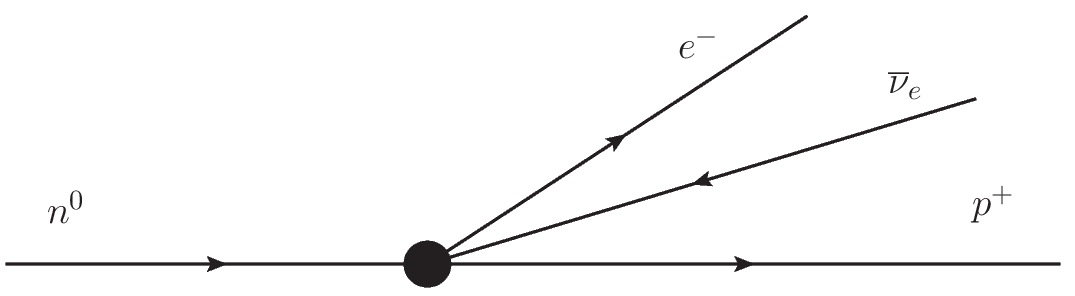
\includegraphics[width=0.9\linewidth]{Images/fourFermi_BetaDecay.png}
	  			\caption{Beschreibung des $\beta$-Zerfalls nach Fermi \cite{fermi_four}.}
	  			\label{fig:fermi}
			\end{figure}
\end{frame}

\begin{frame}{Die Fermi-Wechselwirkung als effektive Theorie}
	\begin{figure}
	  	\centering
		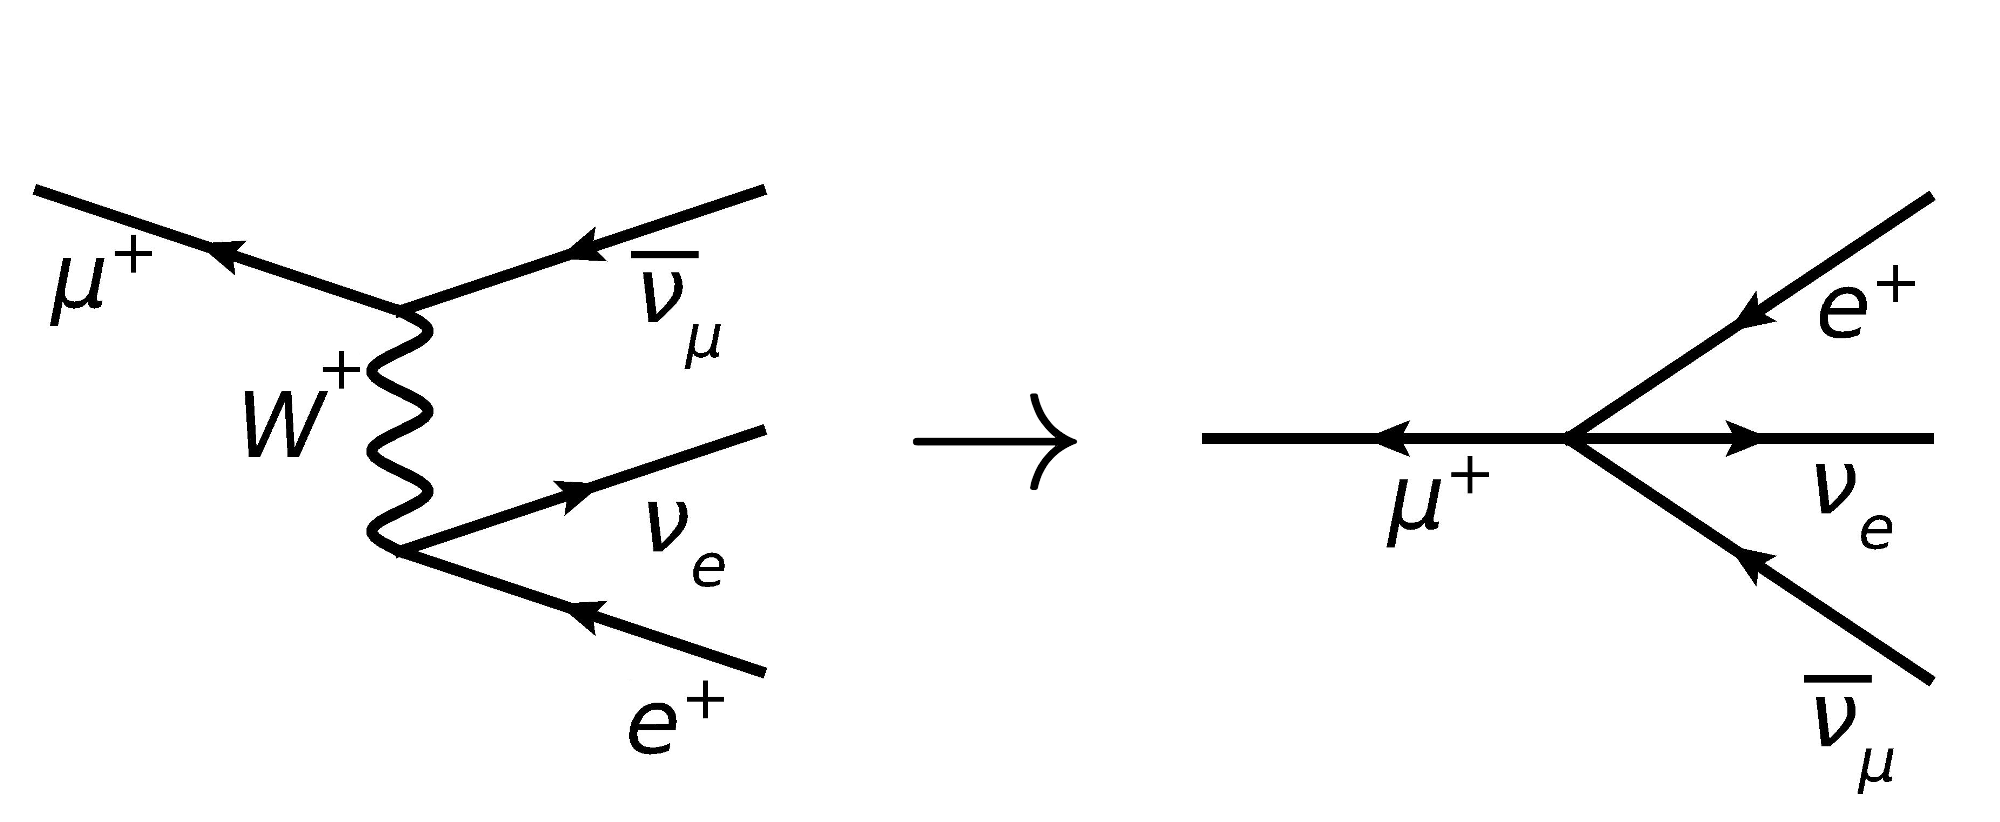
\includegraphics[width=0.8\linewidth]{Images/muon_decay.png}
	  	\label{fig:fermi_2}
	\end{figure}	
		\vspace*{-10px}
	\begin{columns}
		\column{0.45\textwidth}
				{\Large
				\begin{align*}
					\frac{-i \left( g_{\mu\nu} - \frac{q_\mu q_\nu}{M^2} \right)}{q^2 - M^2}
				\end{align*}
				}%
		\column{0.1\textwidth}
				{\LARGE
				\begin{align*}
					\underbrace{\rightarrow}_{q^2 \ll M^2}
				\end{align*}
				}%
		\column{0.45\textwidth}
				{\Large
				\begin{align*}
					\frac{i g_{\mu\nu}}{M^2}
				\end{align*}
				}%
	\end{columns}
	\vspace*{15px}
	\cite{Gorringe:2015cma} (bearbeitet), \cite{Griffiths:111880}
\end{frame}

\begin{frame}{Die Fermi-Wechselwirkung als effektive Theorie}
	\begin{columns}
		\column{0.6\textwidth}
			\begin{itemize}
				\setlength\itemsep{0.5em}
				\item Fermi-Wechselwirkung stellt für kleine Energien (bis heute) eine sehr gute Näherung dar (da schwache Wechselwirkung mit geringer Reichweite)
				\item Verallgemeinerung: Anwendung der Theorie auf viele weitere Reaktionen (z.B. $\mu$-Zerfall) liefert hervorragende Ergebnisse
				\item [$\rightarrow$] Erweiterung der Theorie, um neue Phänomene wie die Paritätsverletzung beschreiben zu können (V-A-Struktur)
			\end{itemize}
		\column{0.4\textwidth}
			\begin{figure}
	  			\centering
				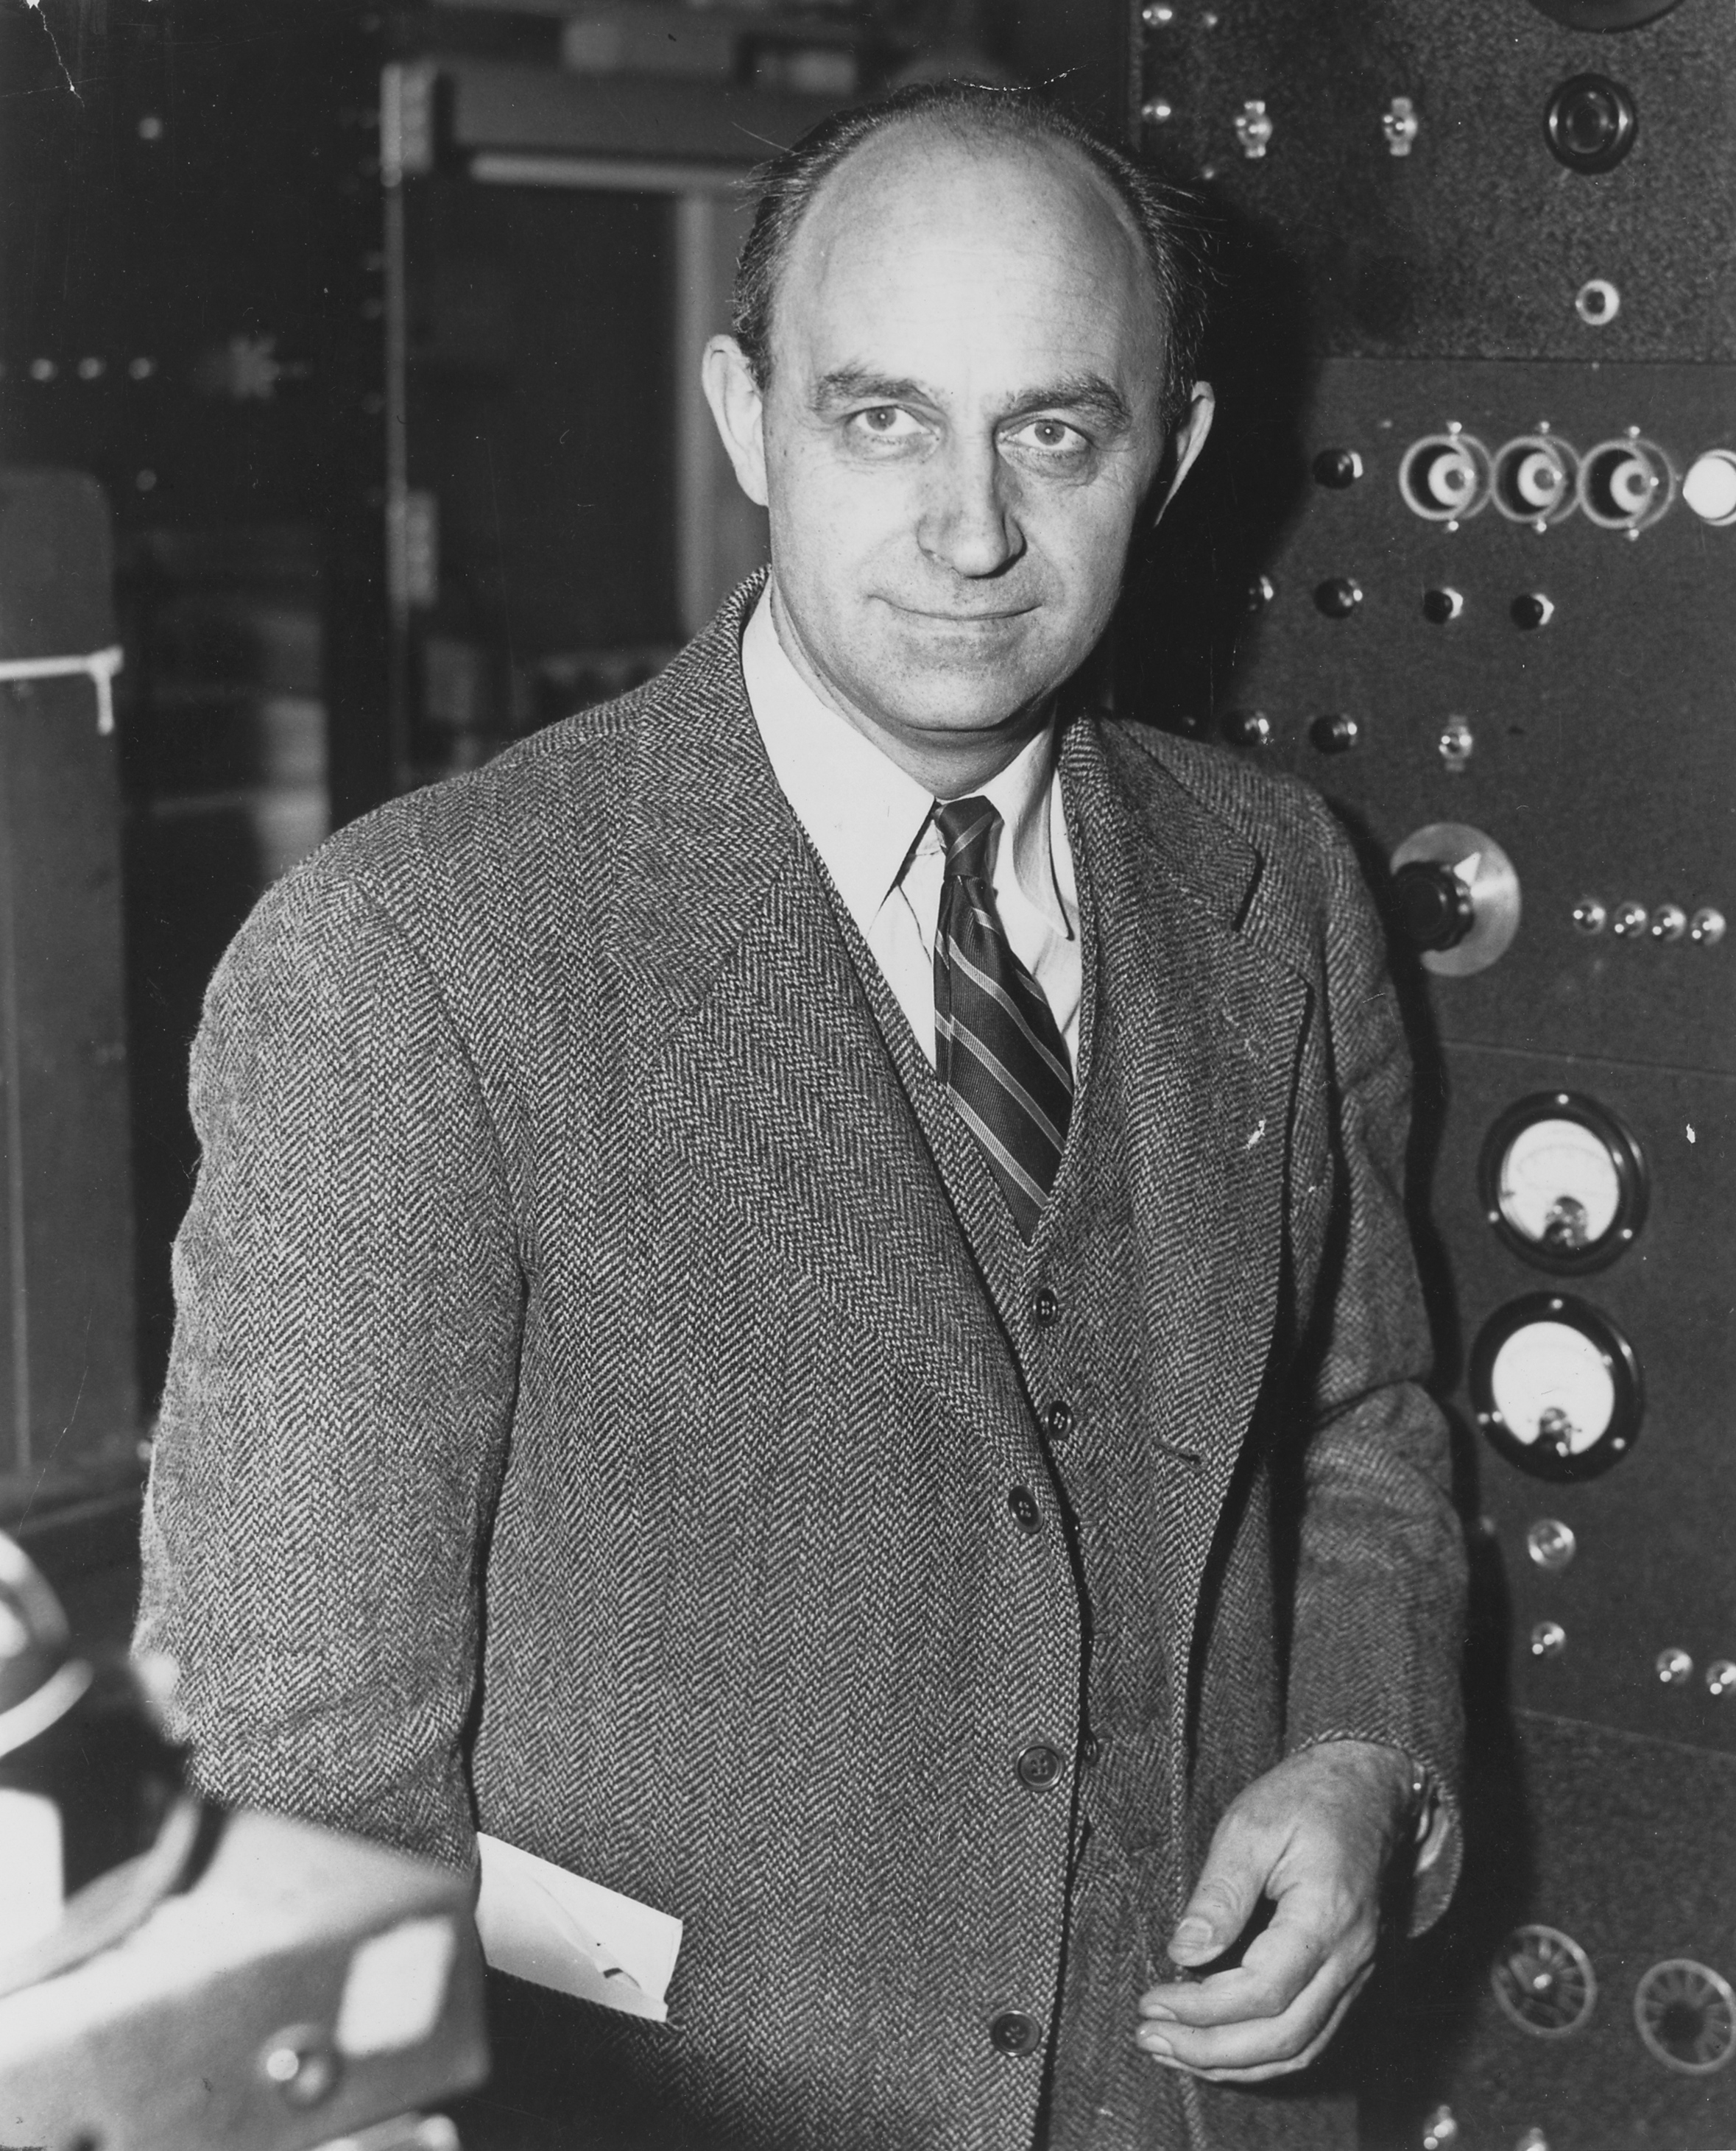
\includegraphics[width=\linewidth]{Images/Enrico_Fermi_1943-49.jpg}
	  			\caption{Enrico Fermi \cite{wiki:fermi}.}
	  			\label{fig:fermi}
			\end{figure}
	\end{columns}
\end{frame}


\begin{frame}{Die Fermi-Wechselwirkung als effektive Theorie}
	\begin{columns}
		\column{0.6\textwidth}
			\begin{itemize}
				\setlength\itemsep{0.5em}
				\item Theorie der Fermi-Wechselwirkung nicht renormierbar
				\item [$\rightarrow$] Divergenzen bei höheren Energien bzw. höheren Ordnungen in $G_\text{F}$
			\end{itemize}
				\vspace*{10px}
			\begin{itemize}
				\item Ab $E \approx \SI{300}{\giga\electronvolt}$: Verletzung des "Unitarity limit"
				\item [$\rightarrow$] $\sigma \propto G_\text{F}^2 E^2$
				\item [$\rightarrow$] Bedingung an totalem Wirkungsquerschnitt, welche aus der Unitarität stammt, wird verletzt (unphysikalisch) \cite{perkins_2000}
			\end{itemize}
			\vspace*{10px}
			\begin{itemize}
				\item Mit höheren Beschleunigerenergien können Abweichungen von der Theorie gemessen werden
			\end{itemize}
		\column{0.4\textwidth}
			\begin{figure}
	  			\centering
				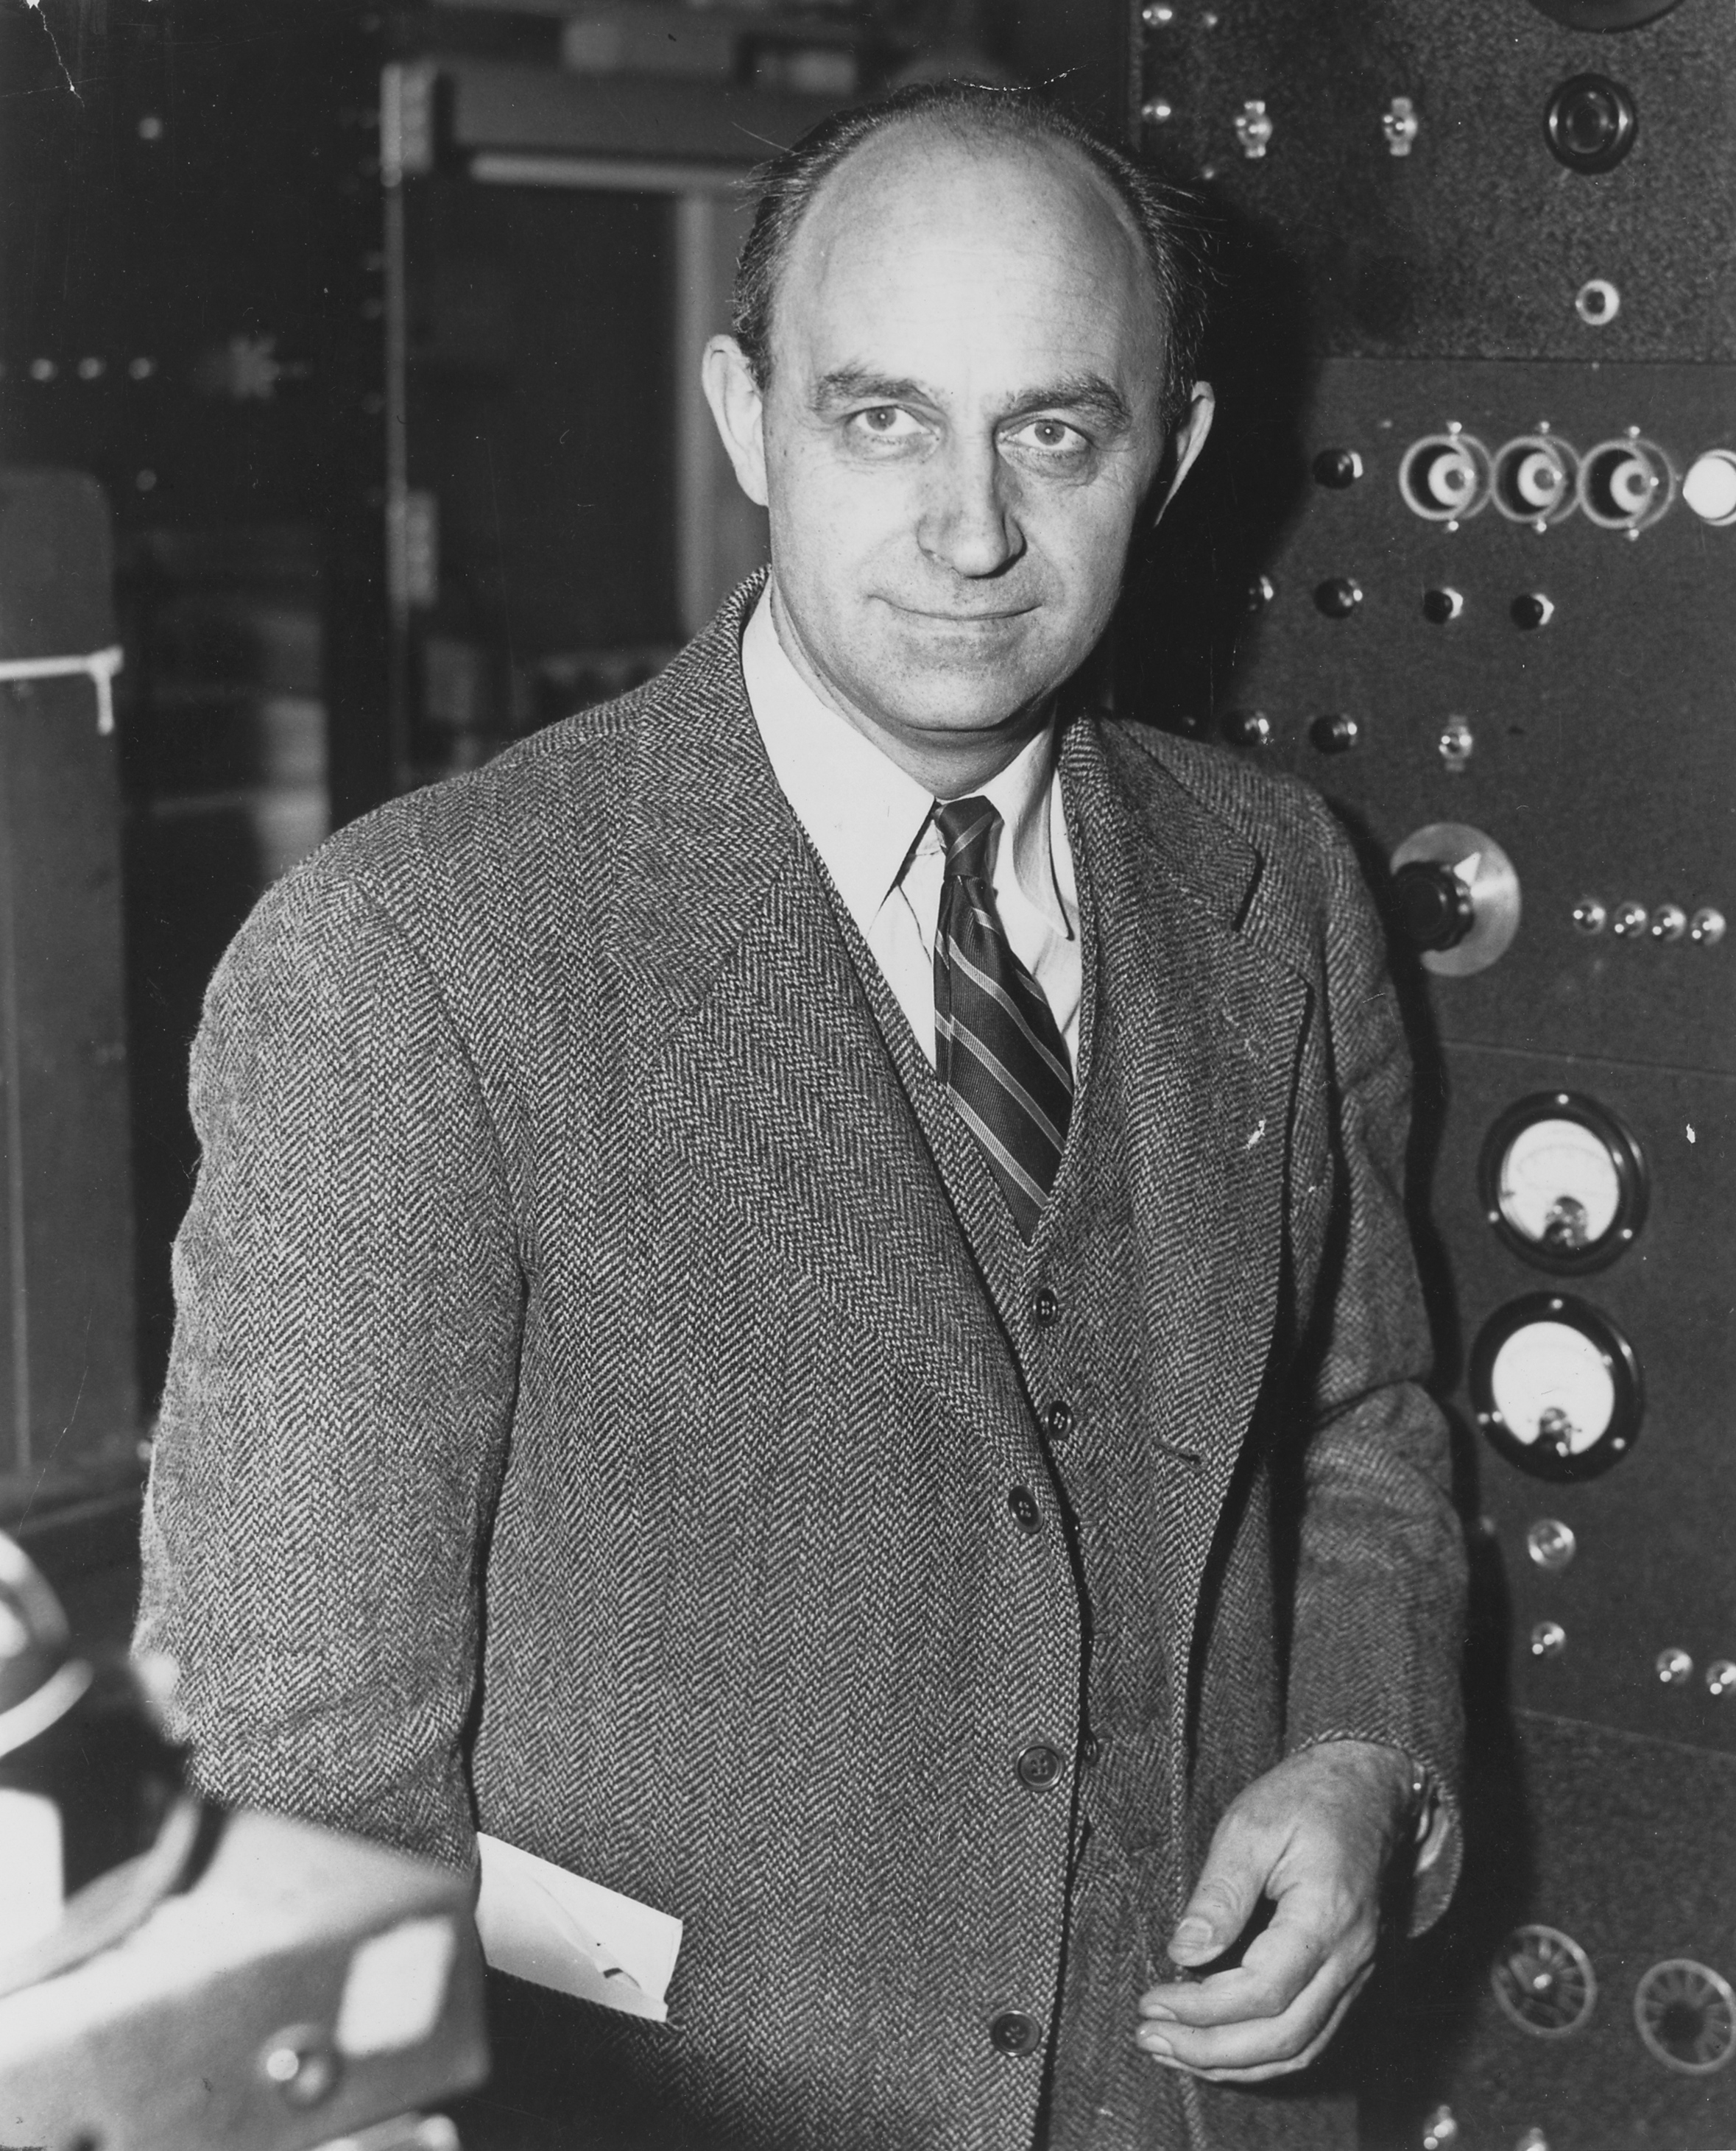
\includegraphics[width=\linewidth]{Images/Enrico_Fermi_1943-49.jpg}
	  			\caption{Enrico Fermi \cite{wiki:fermi}.}
	  			\label{fig:fermi}
			\end{figure}
	\end{columns}
\end{frame}

\begin{frame}{Die elektroschwache Wechselwirkung}
	\begin{columns}
		\column{0.27\textwidth}
			\begin{figure}
	  			\centering
				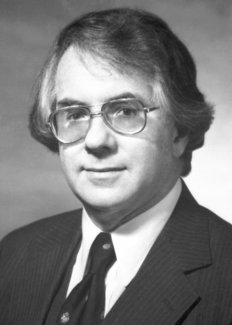
\includegraphics[width=\linewidth]{Images/glashow-13318-content-portrait-mobile-tiny.jpg}
	  			\caption{Sheldon Glashow}
	  			\label{fig:fermi}
			\end{figure}
				\column{0.27\textwidth}
			\begin{figure}
	  			\centering
				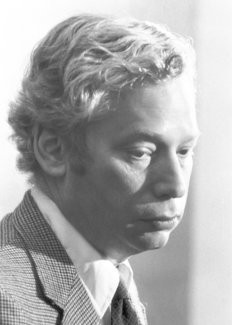
\includegraphics[width=\linewidth]{Images/weinberg-13320-content-portrait-mobile-tiny.jpg}
	  			\caption{Steven Weinberg}
	  			\label{fig:fermi}
			\end{figure}
				\column{0.27\textwidth}
			\begin{figure}
	  			\centering
				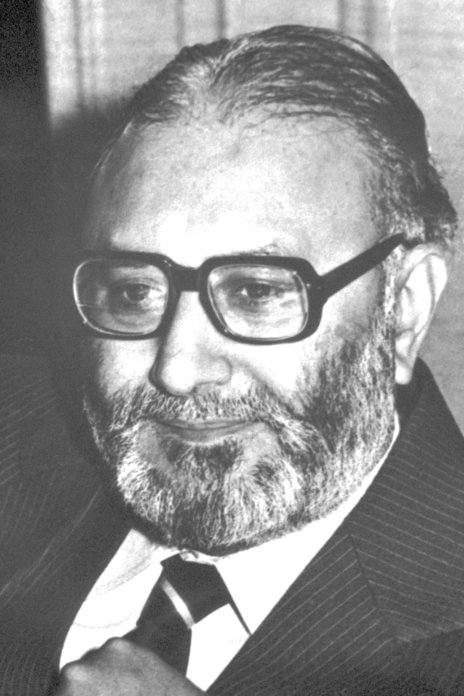
\includegraphics[width=\linewidth]{Images/salam-13319-portrait-mini-2x.jpg}
	  			\caption{Abdus Salam}
	  			\label{fig:fermi}
			\end{figure}
	\end{columns}
	\cite{9789810207274}
\end{frame}

\begin{frame}{Die elektroschwache Wechselwirkung}
			\begin{itemize}
				\setlength\itemsep{0.5em}
				\item \textbf{1968} wird die elektroschwache Wechselwirkung durch Sheldon Glashow, Steven Weinberg und Abdus Salam beschrieben
				\item Vereinheitlichte Theorie der Quantenelektrodynamik und schwachen Wechselwirkung
				\item Vier Austauschteilchen:
				\item [$\rightarrow$] Das masselose Photon $\gamma$
				\item [$\rightarrow$] Die massebehafteten Teilchen $W^+$, $W^-$, $Z^0$
				\item Geringe Stärke und Reichweite der schwachen Wechselwirkung wird begründet durch die hohen Massen der Austauschteilchen
				\item Schwacher Mischungswinkel $\Theta_\text{W}$ als freier Parameter
			\end{itemize}

\end{frame}


\section{Die Entdeckung der neutralen Ströme}

\begin{frame}{Neutrale Ströme (NC)}
	\begin{columns}
		\column{0.5\textwidth}
				\begin{itemize}
					  \setlength\itemsep{0.5em}
					\item Vorhersage der schwachen Ströme durch die elektroschwache Wechselwirkung
				\end{itemize}
				\vspace*{20px}
				\begin{itemize}
					\setlength\itemsep{0.5em}
					\item Leptonische NC: $\nu_\mu + e^- \rightarrow \nu_\mu + e^-$
					\item[$\rightarrow$] Signatur: Einzelnes Elektron
					\item Hadronische NC: $\nu_\mu + N \rightarrow \nu_\mu + X$
					\item[$\rightarrow$] Signatur: Nur Hadronen, ohne Leptonen
				\end{itemize}
		\column{0.5\textwidth}
			\begin{figure}
	  			\centering
				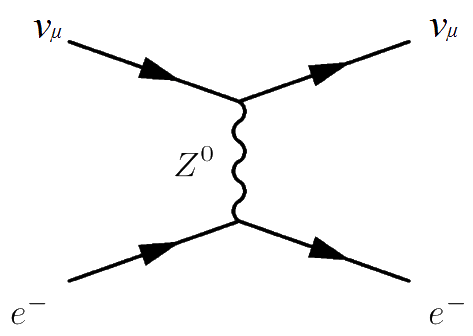
\includegraphics[width=\linewidth]{Images/Neutral_current,_leptonic_event,_muon_neutrino.png}
	  			\caption{Feynman-Diagramm eines leptonischen neutralen Stromes \cite{wiki:NC}.}
	  			\label{fig:feynman}
			\end{figure}
	\end{columns}
\end{frame}

\begin{frame}
	\begin{figure}
	  \centering
	  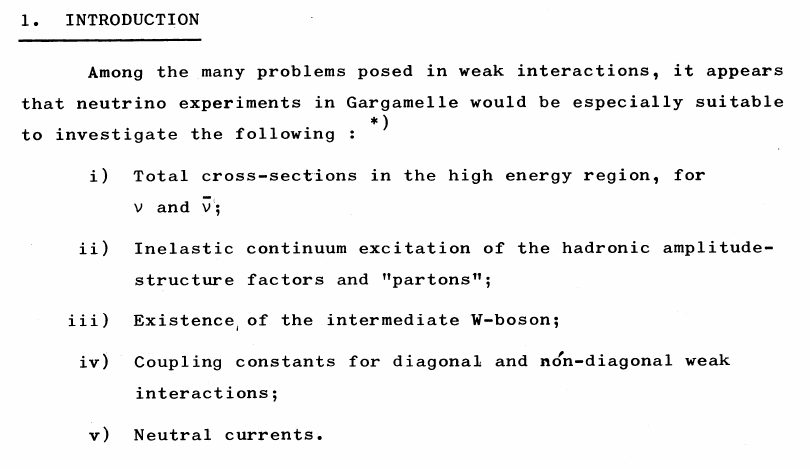
\includegraphics[width=0.9\linewidth]{Images/Screenshot_2018-11-26_16-27-27.png}
	  \caption{Auszug aus dem Proposal zum Gargamelle Detektor, März 1970 \cite{proposal}.}
	  \label{fig:proposal}
	\end{figure}
\end{frame}

\begin{frame}{Der Gargamelle Detektor}
	\begin{columns}
		\column{0.6\textwidth}
				\begin{itemize}
					\setlength\itemsep{0.5em}
					\item Blasenkammer, betrieben am CERN von 1970 bis 1979
					\item[$\rightarrow$] Kammer gefüllt mit \SI{12}{\cubic\metre} Freon ($\ce{CBrF3}$)
					\item[$\rightarrow$] Temperatur der Flüssigkeit über der Siedetemperatur
					\item[$\rightarrow$] Durchquerende Teilchen ionisieren die Flüssigkeit, wobei Dampfblasen entstehen
					\item[$\rightarrow$] Nachweis der Gasblasen durch Kameras
					\item Kammer \SI{4.8}{\meter} lang, \SI{2}{\meter} im Durchmesser, \SI{2}{\tesla} Magnetfeld (zur Rekonstruktion)
				\end{itemize}

		\column{0.4\textwidth}
			\begin{figure}
	  			\centering
				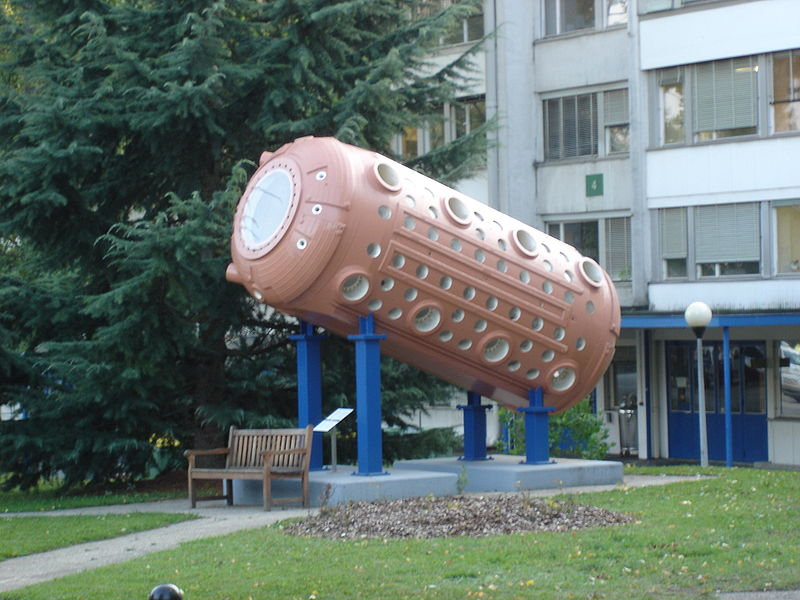
\includegraphics[width=\linewidth]{Images/800px-Gargamelle.jpg}
	  			\caption{Gargamelle Blasenkammer, ausgestellt am CERN \cite{wiki:gargamelle}.}
	  			\label{fig:feynman}
			\end{figure}
	\end{columns}
\end{frame}

\begin{frame}{Der Gargamelle Detektor - Neutrinoquelle}
	\begin{columns}
		\column{0.6\textwidth}
				\begin{itemize}
					\setlength\itemsep{0.5em}
					\item Als Neutrinoquelle diente ein Protonenbeam vom Proton Syncrotron (\SI{26}{\giga\electronvolt})
					\item[$\rightarrow$] Entstehung von Kaonen und Pionen durch Kollision der Protonen mit einem Beryllium-Target
					\item[$\rightarrow$] Kaonen und Pionen werden fokussiert und zerfallen in einem \SI{70}{\metre} langen Tunnel in Myonen und Neutrinos
					\item[$\rightarrow$] Neutrinoenergie im Bereich \SI{1}{\giga\electronvolt} bis \SI{10}{\giga\electronvolt}
				\end{itemize}

		\column{0.4\textwidth}
			\begin{figure}
	  			\centering
				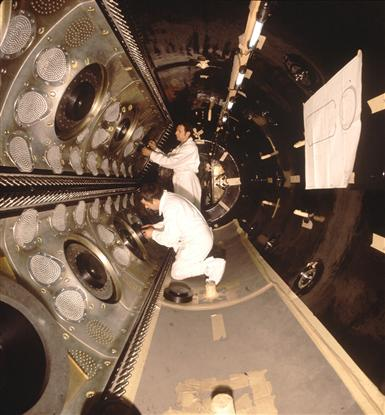
\includegraphics[width=\linewidth]{Images/7011042-A5-at-72-dpi.jpg}
	  			\caption{Blick in die Gargamelle Blasenkammer \cite{CERN-EX-7011042}.}
	  			\label{fig:feynman}
			\end{figure}
	\end{columns}
\end{frame}

\begin{frame}{Der Gargamelle Detektor - Erste Resultate}
	\begin{columns}
		\column{0.6\textwidth}
				\begin{itemize}
					\setlength\itemsep{0.5em}
					\item \textbf{März 1972}: Erste Hinweise auf hadronische schwache Ströme ändern die Prioritäten der Analyse
					\item[$\rightarrow$] Suche sowohl nach hadronischen als auch leptonischen Events
					\item[$\rightarrow$] Leptonische Events: Weniger Hintergrundereignisse, treten jedoch selten auf
					\item \textbf{Dezember 1972}: Erste Beobachtung eines leptonischen NC-Events
					\item \textbf{19. Juli 1973}: Entdeckung der schwachen Ströme (leptonisch und hadronisch) wird präsentiert
				\end{itemize}

		\column{0.4\textwidth}
			\begin{figure}
	  			\centering
				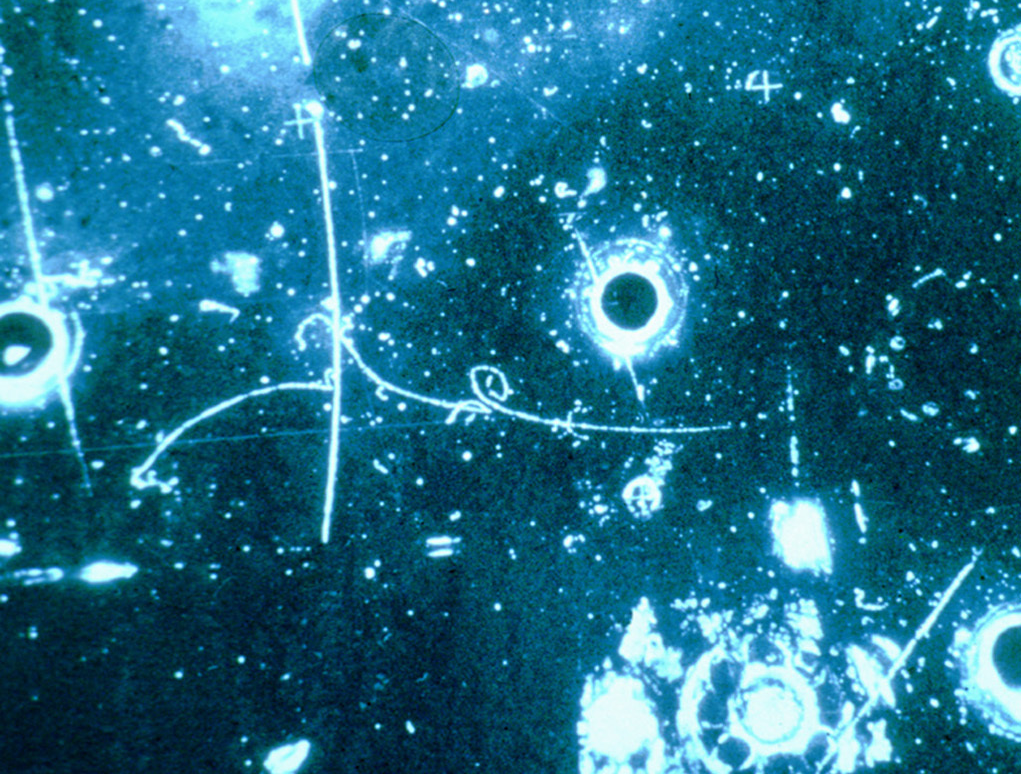
\includegraphics[width=\linewidth]{Images/60100_bearbeitet.png}
	  			\caption{Beobachtung eines leptonischen neutralen Stromes \cite{CERN-EX-60100}. Das Elektron bewegt sich horizontal von rechts nach links.}
	  			\label{fig:feynman}
			\end{figure}
	\end{columns}
\end{frame}

\begin{frame}{Der Gargamelle Detektor - Erste Resultate}
		\begin{itemize}
			\setlength\itemsep{0.5em}
			\item Aus den Ergebnissen des Experimentes konnten die Massen von W-Boson und Z-Boson vorhergesagt werden \cite{doi:10.1142/9789814644150_0006}:
			\begin{align*}
				M_W &\approx \left(60-80\right)\si{\giga\electronvolt}\\
				M_Z &\approx \left(75-92\right)\si{\giga\electronvolt}
			\end{align*}
			\item Jedoch existierte noch kein Experiment, welches die zur Erzeugung notwendige Schwerpunktsenergie zur Verfügung stellen konnte
			\item[$\Rightarrow$]Verschieben der "energy frontier" notwendig!

		\end{itemize}
		\end{frame}

%
%------------------------------------------------

\begin{frame}[focus]
	Vielen Dank für die Aufmerksamkeit!
\end{frame}

%----------------------------------------------------------------------------------------
%	 CLOSING/SUPPLEMENTARY SLIDES
%----------------------------------------------------------------------------------------

\appendix

\begin{frame}[allowframebreaks]{References}
	\bibliography{example.bib}
	\bibliographystyle{plain}
\end{frame}

%------------------------------------------------

\begin{frame}{Backup Slide}
	This is a backup slide, useful to include additional materials to answer questions from the audience.
	\vfill
	The package \texttt{appendixnumberbeamer} is used to refrain from numbering appendix slides.
\end{frame}

%----------------------------------------------------------------------------------------

\end{document}
